%% Do not edit preable unless you know what you are doing.
\documentclass{article}\usepackage[]{graphicx}\usepackage[]{color}
% maxwidth is the original width if it is less than linewidth
% otherwise use linewidth (to make sure the graphics do not exceed the margin)
\makeatletter
\def\maxwidth{ %
  \ifdim\Gin@nat@width>\linewidth
    \linewidth
  \else
    \Gin@nat@width
  \fi
}
\makeatother

\definecolor{fgcolor}{rgb}{0.345, 0.345, 0.345}
\newcommand{\hlnum}[1]{\textcolor[rgb]{0.686,0.059,0.569}{#1}}%
\newcommand{\hlstr}[1]{\textcolor[rgb]{0.192,0.494,0.8}{#1}}%
\newcommand{\hlcom}[1]{\textcolor[rgb]{0.678,0.584,0.686}{\textit{#1}}}%
\newcommand{\hlopt}[1]{\textcolor[rgb]{0,0,0}{#1}}%
\newcommand{\hlstd}[1]{\textcolor[rgb]{0.345,0.345,0.345}{#1}}%
\newcommand{\hlkwa}[1]{\textcolor[rgb]{0.161,0.373,0.58}{\textbf{#1}}}%
\newcommand{\hlkwb}[1]{\textcolor[rgb]{0.69,0.353,0.396}{#1}}%
\newcommand{\hlkwc}[1]{\textcolor[rgb]{0.333,0.667,0.333}{#1}}%
\newcommand{\hlkwd}[1]{\textcolor[rgb]{0.737,0.353,0.396}{\textbf{#1}}}%
\let\hlipl\hlkwb

\usepackage{framed}
\makeatletter
\newenvironment{kframe}{%
 \def\at@end@of@kframe{}%
 \ifinner\ifhmode%
  \def\at@end@of@kframe{\end{minipage}}%
  \begin{minipage}{\columnwidth}%
 \fi\fi%
 \def\FrameCommand##1{\hskip\@totalleftmargin \hskip-\fboxsep
 \colorbox{shadecolor}{##1}\hskip-\fboxsep
     % There is no \\@totalrightmargin, so:
     \hskip-\linewidth \hskip-\@totalleftmargin \hskip\columnwidth}%
 \MakeFramed {\advance\hsize-\width
   \@totalleftmargin\z@ \linewidth\hsize
   \@setminipage}}%
 {\par\unskip\endMakeFramed%
 \at@end@of@kframe}
\makeatother

\definecolor{shadecolor}{rgb}{.97, .97, .97}
\definecolor{messagecolor}{rgb}{0, 0, 0}
\definecolor{warningcolor}{rgb}{1, 0, 1}
\definecolor{errorcolor}{rgb}{1, 0, 0}
\newenvironment{knitrout}{}{} % an empty environment to be redefined in TeX

\usepackage{alltt}
\usepackage[sc]{mathpazo}
\usepackage[T1]{fontenc}
\usepackage[english]{babel}
\usepackage[utf8]{inputenc}
\usepackage{geometry}
\usepackage{dsfont}
\usepackage{indentfirst}
\usepackage{fancyhdr}
\usepackage{amsmath}
\usepackage{amssymb}
\usepackage{enumitem}

% No indents in whole document
\setlength\parindent{0pt}

% Gaps between item is itemize
\setitemize{itemsep=-1em,topsep=0.5em,parsep=0em,partopsep=0pt}

% Margins of the document
\geometry{verbose,tmargin=2.5cm,bmargin=2.5cm,lmargin=2.5cm,rmargin=2.5cm}

% Header and footer for all pages
\pagestyle{fancy}
\fancyhf{}
\renewcommand{\headrulewidth}{0pt}
\rfoot{Page \thepage}

% Header and footer for first page
\fancypagestyle{plain}{%
  \renewcommand{\headrulewidth}{0pt}%
  \fancyhf{}%
  \rhead{ETH Zurich}
  \lhead{Applied Generalized Linear Models \\ Spring Semester 2020}
  \rfoot{Page \thepage}
}

% Global Settings of R-code


% Mathematics Operators for Ease of Notation
\DeclareMathOperator{\SSR}{SSR}
\DeclareMathOperator{\SSreg}{SSreg}
\DeclareMathOperator{\SST}{SST}

% Bad Box settings
\hbadness=10000
\vbadness=\maxdimen
\vfuzz=30pt
\hfuzz=30pt


%% ---------- BEGIN DOCUMENT -----------------------------------------------
\IfFileExists{upquote.sty}{\usepackage{upquote}}{}
\begin{document}
%\SweaveOpts{concordance=TRUE}

%% Tiltle
\title{Assignment 1}
\author{Milan Kuzmanovic, Mark McMahon \\ Martin Kotuliak, Jakub Polak}
\date{\today}
\maketitle

\section*{Task 1}

A multiple linear regression model has been estimated to study the relationship between $Y =$ violent crime rate (per 100,000 people), $X_1 =$ poverty rate (percentage with income below the poverty line) and $X_2 =$ percentage living in urban area. Data are collected in 51 cities in the U.S.\\

1)
The relevant equations that relate estimates, standard error, T-statistic, R-squared and Sum of Squares of residuals (SSR), regression (SSReg), and total (SST) are the following:

  \[ \frac{\hat{\beta_j}}{se(\hat{\beta_j})} = t-value \qquad R^2 = \frac{\SSreg}{\SST}= 1-\frac{\SSR}{\SST}  \qquad \SST = \SSreg + \SSR
\]

We plug in the corresponding information that is already provided and compute the missing values.

\begin{knitrout}
\definecolor{shadecolor}{rgb}{0.969, 0.969, 0.969}\color{fgcolor}\begin{kframe}
\begin{alltt}
\hlstd{a} \hlkwb{<-} \hlopt{-}\hlnum{498.683} \hlopt{/} \hlnum{140.988}
\hlstd{b} \hlkwb{<-} \hlnum{4.885} \hlopt{*} \hlnum{6.677}
\hlstd{c} \hlkwb{<-} \hlnum{9.112} \hlopt{/} \hlnum{6.900}
\hlstd{d} \hlkwb{<-} \hlnum{1841257.15} \hlopt{/} \hlstd{(}\hlnum{1} \hlopt{-} \hlnum{0.5708}\hlstd{)}
\hlstd{e} \hlkwb{<-} \hlstd{d} \hlopt{-} \hlnum{1841257.15}
\end{alltt}
\end{kframe}
\end{knitrout}

The table below reports the output with filled in missing information.

\begin{center}
\begin{tabular}{ l r r r r }
 \hline
            & Est.            & s.e.              & t-value         & p-value \\
 \hline
 Intercept  & -498.683  & 140.988 & $^{a\;}$-3.537 & 0.009 \\
 $X_1$      & $^{b\;}$32.617 & 6.677  & 4.885     & 0.001 \\
 $X_2$      & 9.112  & $^{c\;}$1.321 & 6.900      & 0.001 \\
 \hline
 $R^2$      & 0.5708            & & & \\
 SSreg      & $^{e\;}$2448717.57 & & & \\
 SSR        & 1841257.15        & & & \\
 SSTotal    & $^{d\;}$4289974.72 & & & \\
 \hline
\end{tabular}
\end{center}

2)
The coefficient of determination $R^2$ is equal to $0.5708$. This value measures the proportion of the variance in $Y$ explained by the fitted model. Hence, 57.08 \% of the sample variability of $Y$ can be explained by the linear combination of given $X_j$'s for the given data sample. \\

3)
The global F-test tests a null hypothesis that all regression coefficients are simultaneously 0. In a mathematical notation, $H_0 : \beta_1 = \beta_2 = 0$. To evaluate the overall F-test we use the statistic in the equation below which has, under the above null hypothesis, F-distribution with corresponding degrees of freedom.
\[ F = \frac{\SSreg/p}{\SSR/(n-(p+1))} \sim F_{p,n-(p+1)}
\]

The data are collected in 51 cities, so $n=51$ and we have 2 predictors, so $p=2$. Other values we can easily obtain from the filled table above.
\begin{knitrout}
\definecolor{shadecolor}{rgb}{0.969, 0.969, 0.969}\color{fgcolor}\begin{kframe}
\begin{alltt}
\hlstd{(f} \hlkwb{=} \hlstd{(e} \hlopt{/} \hlnum{2}\hlstd{)} \hlopt{/} \hlstd{(}\hlnum{1841257.15} \hlopt{/} \hlstd{(}\hlnum{51}\hlopt{-}\hlstd{(}\hlnum{2}\hlopt{+}\hlnum{1}\hlstd{)) ))}
\end{alltt}
\begin{verbatim}
## [1] 31.91799
\end{verbatim}
\end{kframe}
\end{knitrout}

Hence, the F-statistic has a value of 31.917987. To evaluate the test, and decide on whether we reject or accept $H_0$, we can compute its p-value. The p-value represents the probability of observing equal or more extreme value than the observed F-statistic, for the corresponding F-distribution under the null hypothesis. We reject the null hypothesis if the p-value is lower than the pre-determined significance level of the test $\alpha$, which is generally chosen to be $\alpha = 0.05$

\begin{knitrout}
\definecolor{shadecolor}{rgb}{0.969, 0.969, 0.969}\color{fgcolor}\begin{kframe}
\begin{alltt}
\hlstd{(p} \hlkwb{=} \hlkwd{pf}\hlstd{(f,}\hlnum{2}\hlstd{,}\hlnum{48}\hlstd{,}\hlkwc{lower.tail} \hlstd{=} \hlnum{FALSE}\hlstd{))}
\end{alltt}
\begin{verbatim}
## [1] 1.526979e-09
\end{verbatim}
\end{kframe}
\end{knitrout}

The p-value is \ensuremath{1.5269792\times 10^{-9}}, which is lower than the standard significance level $\alpha=0.05$ and therefore, we can reject the null hypothesis $H_0 : \beta_1 = \beta_2 = 0$. In other words, there is a significant evidence against the null hypothesis that all regression coefficients are simultaneously zero. Hence, the model with all the covariates is better than the one with just the intercept. This test indicates that the linear model is suitable to explain significant portion of the variance in the outcome variable.

\section*{Task 2}

The table below shows the scores of the first test (maximum score 10 points) in a beginning German course. Students in the course are grouped as follows:
\begin{itemize}
\item Group A: Never studied foreign language before, but have good English skills\\
\item Group B: Never studied foreign language before, have poor English skills\\
\item Group C: Studied other foreign language
\end{itemize}

\begin{center}
\begin{tabular}{ c c c }
 \hline
 Group A & Group B & Group C \\
 \hline
 4 & 1 & 9 \\
 6 & 5 & 10 \\
 8 &   & 5 \\
 \hline
\end{tabular}
\end{center}

1)
The aim is to compare means of the different groups. If we would be comparing only two groups, we would use two-sample t-test. For the situation where there is more than two groups, identified by a factor we can the one-way/one-factor analysis of variance (ANOVA). This corresponds to our situation and it tests if at least one group is different than others.\\

The Assumptions of the ANOVA are following:
\begin{itemize}
\item The observations ${y_{ij}}$ represent $N$ iid realizations of the data generating process $Y_{ij} = \mu + \alpha_j + \epsilon_{ij}$; \\
\item Errors $\epsilon_{ij}$ are iid and normally distributed, i.e. $\epsilon_{ij} \sim \mathcal{N}(0, \sigma^2)$ which implies that $Y_{ij} \sim \mathcal{N}(\mu + \alpha_j, \sigma^2)$ for every group $j = 1,...,M$.
\end{itemize}

The Hypothesis tested in ANOVA is the following:
\begin{itemize}
\item Null hypothesis: the means of the different groups are equal, i.e. $H_0 : \mu_1 = \mu_2 = ... = \mu_M$; \\
\item Alternative hypothesis: At least one group mean is different than the others.
\end{itemize}

The F-test is used for testing the null hypothesis that all of the group means are equal. In ANOVA, the F-statistic is computed as the ratio of the variance between groups ($SSReg = \sum_{j = 1}^{M} n_j (\bar{y_j} - \bar{y})^2)$) and variance within groups ($SSR = \sum_{j = 1}^{M} \sum_{i = 1}^{n_j} (y_{ij} - \bar{y_j})^2)$), both divided by the corresponding degrees of freedom. Intuitively, the larger is the variance between groups relative to the variance within groups, the more evidence we have against the null hypothesis that the group means are equal. Formally, the F-statistic under the null hypothesis is given by:
\[ F = \frac{\SSreg/(M - 1)}{\SSR/(N - M)} \sim F_{M - 1,N - M}
\]
We reject the null hypothesis when the value of the F-statistic is large. More specifically, we compute the p-value, i.e. the probability of observing equal or more extreme value than the observed F-statistic, for the corresponding F-distribution under the null hypothesis, and then we reject the null hypothesis if the p-value is lower than the pre-determined significance level $\alpha$, with $\alpha = 0.05$ in general.
\\

In the example above we have three groups, i.e. $M = 3$ and eight data points, $N = 8$.With the code below, we specify the data and compute common statistics for each group.
\begin{knitrout}
\definecolor{shadecolor}{rgb}{0.969, 0.969, 0.969}\color{fgcolor}\begin{kframe}
\begin{alltt}
\hlstd{X} \hlkwb{<-} \hlkwd{data.frame}\hlstd{(}\hlstr{"grade"} \hlstd{=} \hlkwd{c}\hlstd{(}\hlnum{4}\hlstd{,}\hlnum{6}\hlstd{,}\hlnum{8}\hlstd{,}\hlnum{1}\hlstd{,}\hlnum{5}\hlstd{,}\hlnum{9}\hlstd{,}\hlnum{10}\hlstd{,}\hlnum{5}\hlstd{),}
                \hlstr{"group"} \hlstd{=} \hlkwd{c}\hlstd{(}\hlstr{"A"}\hlstd{,}\hlstr{"A"}\hlstd{,}\hlstr{"A"}\hlstd{,}\hlstr{"B"}\hlstd{,}\hlstr{"B"}\hlstd{,}\hlstr{"C"}\hlstd{,}\hlstr{"C"}\hlstd{,}\hlstr{"C"}\hlstd{))}

\hlkwd{library}\hlstd{(dplyr)}
\hlkwd{data.frame}\hlstd{(}\hlkwd{group_by}\hlstd{(X, group)} \hlopt
  \hlkwd{summarise}\hlstd{(} \hlkwc{count} \hlstd{=} \hlkwd{n}\hlstd{(),} \hlkwc{mean} \hlstd{=} \hlkwd{mean}\hlstd{(grade),} \hlkwc{var} \hlstd{=} \hlkwd{var}\hlstd{(grade),} \hlkwc{sd} \hlstd{=} \hlkwd{sd}\hlstd{(grade)))}
\end{alltt}
\begin{verbatim}
##   group count mean var       sd
## 1     A     3    6   4 2.000000
## 2     B     2    3   8 2.828427
## 3     C     3    8   7 2.645751
\end{verbatim}
\end{kframe}
\end{knitrout}

These can be easily visualised with a boxplot (left) or a group means plot with errorbars signifying one standard deviation (right). The main observation we conclude from these plots is the large estimated variance within groups, which is caused mainly by having just a few observations.

\begin{knitrout}
\definecolor{shadecolor}{rgb}{0.969, 0.969, 0.969}\color{fgcolor}

{\centering 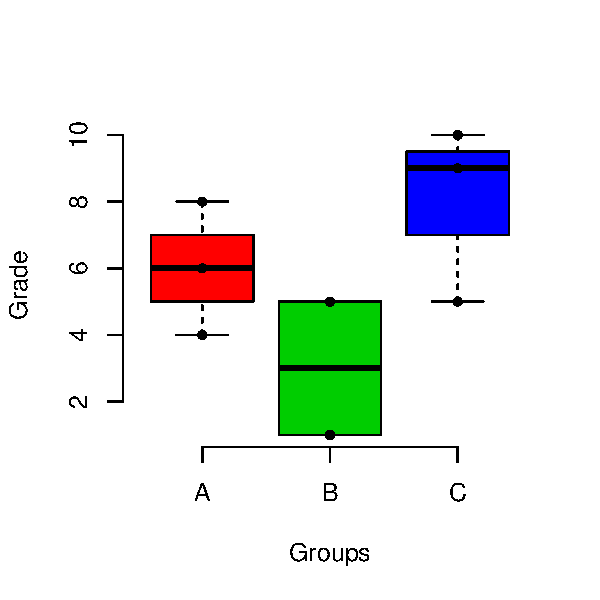
\includegraphics[width=.4\linewidth]{figures/plot-t2-plots-1} 
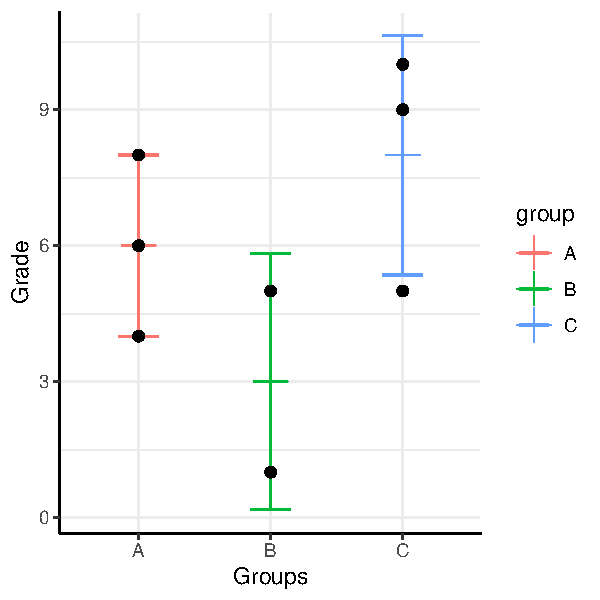
\includegraphics[width=.4\linewidth]{figures/plot-t2-plots-2} 

}



\end{knitrout}

Finally, below we compute the ANOVA tests with our data using the function \verb+aov()+.

\begin{knitrout}
\definecolor{shadecolor}{rgb}{0.969, 0.969, 0.969}\color{fgcolor}\begin{kframe}
\begin{alltt}
\hlstd{fit} \hlkwb{<-} \hlkwd{aov}\hlstd{(grade} \hlopt{~} \hlstd{group,} \hlkwc{data} \hlstd{= X)}
\hlkwd{summary}\hlstd{(fit)}
\end{alltt}
\begin{verbatim}
##             Df Sum Sq Mean Sq F value Pr(>F)
## group        2     30      15     2.5  0.177
## Residuals    5     30       6
\end{verbatim}
\end{kframe}
\end{knitrout}

The p-value of 0.177 indicates that we cannot reject the null hypothesis that the group means are different at significance level $\alpha = 0.05$, even though the estimated means seem different. The main reason for the lack of evidence against the null hypothesis, despite differences in estimated means, is the high variance in estimation caused by having only a few observations. Intuitively, having small data sample leaves more room for the possibility that the estimated differences happened due to the variance in estimation, and not due to the existance of true differences, and that is why it is harder to reject the null hypothesis that there are no differences. Formally, this uncertainty in the estimation caused by small data sample is quantified by the low degrees of freedom in the denominator of the F-distribution which makes the F-statistic smaller compared to the case when we have more data, and also makes the shape of the F-distribution such that we require higher F-statistic to reject the null hypothesis at given significance level compared to the case when we have more data. \\



Case (2):\\
Suppose that the first observation in the second group was actually 9, not 1. Then, the standard deviations are the same, but the sample means are 6, 7 and 8, rather than 6, 3 and 8. In this situation, we would expect the F-test statistic to be smaller. The main reason is that the numerator of the F-statistic, $SSReg$, which represents the variance between groups, decreases when the estimated group means are closer to each other. \\

Case (3):\\
Suppose you have the same means as these data, but the sample standard deviations were 1.0, 1.8 and 1.6, instead of the actual 2.0, 2.8 and 2.6. In this situation, we would expect the F-test statistic to be larger. The main reason is that the denominator of the F-statistic, $SSR$, which represents the variance within groups, decreases directly when the above decrease in variance within groups happens.\\

Case (4):\\
Suppose you have the same means and standard deviations as these data, but the sample size were 30, 20 and 30, instead of 3, 2 and 3. In this case, we would expect the F-test statistic to be larger. The main reason is that the F-distribution with which we would be comparing our F-test statistic would be with 2 and 77 degrees of freedom. The variance between groups would still has the same number of degrees of freedom because the number of groups hasn't changed. However, the variance within groups would then have 77 degrees of freedom compared to previously having only 5 degrees of freedom. Therefore, we would be dividing $SSR$ by 77 instead of 5, which would result in a signigicantly larger F-statistic.\\

5)
The p-value is defined as the probaility of observing equal or more extreme value that the test statistic for the distribution under the null hypothesis. In the case of F-test, p-value is the probability of observing equal or larger value than the observed F-statistic for the corresponding F-distribution under the null hypothesis. This means that if the F-statistic were to increase, the p-value would decrease because the probability of observing equal or larger value than the F-statistic would decrease. Opposite happens if the F-statistic were to decrease. Therefore, in case (2) we would expect the p-value to increase, and in cases (3) and (4) we would expect p-value to decerase.


\section*{Task 3}

The compressive strength of concrete is being studied, and four different mixing techniques are being investigated. The following data have been collected. For each mixing technique, 4 compressive strength measurements (in pounds per square inch) have been recorded.\\

\begin{center}
\begin{tabular}{ l c c c c}
 \hline
 & \multicolumn{4}{c}{Compressive Strength} \\
 \hline
 Mixing & 1 & 2 & 3 & 4 \\
 \hline
 1 & 3129 & 3000 & 2865 & 2890 \\
 2 & 3200 & 3300 & 2975 & 3150 \\
 3 & 2800 & 2900 & 2985 & 3050 \\
 4 & 2600 & 2700 & 2600 & 2765 \\
 \hline
\end{tabular}
\end{center}

1) In this task we perform the same one-factor Analysis of Variance as in previous task, in order to answer the question of whther the mixing technique has influence on the compressive strength of the concrete. We load the data to R in following way and subsequently visualise it with same techniques as before. From the plots we can clearly see that some mixing techniques are quite different to others.

\begin{knitrout}
\definecolor{shadecolor}{rgb}{0.969, 0.969, 0.969}\color{fgcolor}\begin{kframe}
\begin{alltt}
\hlstd{X} \hlkwb{<-} \hlkwd{data.frame}\hlstd{(}\hlstr{"strength"}\hlstd{=}\hlkwd{c}\hlstd{(}\hlnum{3129}\hlstd{,}\hlnum{3000}\hlstd{,}\hlnum{2865}\hlstd{,}\hlnum{2890}\hlstd{,}
                             \hlnum{3200}\hlstd{,}\hlnum{3300}\hlstd{,}\hlnum{2975}\hlstd{,}\hlnum{3150}\hlstd{,}
                             \hlnum{2800}\hlstd{,}\hlnum{2900}\hlstd{,}\hlnum{2985}\hlstd{,}\hlnum{3050}\hlstd{,}
                             \hlnum{2600}\hlstd{,}\hlnum{2700}\hlstd{,}\hlnum{2600}\hlstd{,}\hlnum{2765}\hlstd{),}
                \hlstr{"mixing"}\hlstd{=}\hlkwd{rep}\hlstd{(}\hlkwd{c}\hlstd{(}\hlstr{"1"}\hlstd{,}\hlstr{"2"}\hlstd{,}\hlstr{"3"}\hlstd{,}\hlstr{"4"}\hlstd{),}\hlkwd{c}\hlstd{(}\hlnum{4}\hlstd{,}\hlnum{4}\hlstd{,}\hlnum{4}\hlstd{,}\hlnum{4}\hlstd{)) )}
\end{alltt}
\end{kframe}
\end{knitrout}


\begin{knitrout}
\definecolor{shadecolor}{rgb}{0.969, 0.969, 0.969}\color{fgcolor}

{\centering 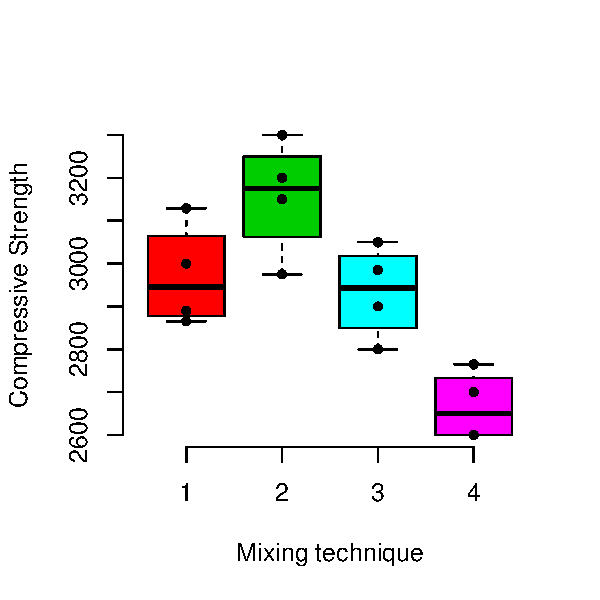
\includegraphics[width=.4\linewidth]{figures/plot-t3-plots-1} 
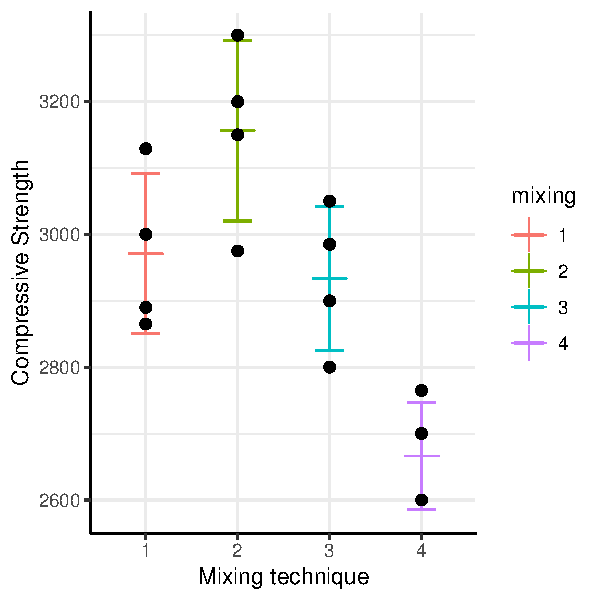
\includegraphics[width=.4\linewidth]{figures/plot-t3-plots-2} 

}



\end{knitrout}

Below, we perform the Analysis of Variance using again \verb+aov()+ function.\\

\begin{knitrout}
\definecolor{shadecolor}{rgb}{0.969, 0.969, 0.969}\color{fgcolor}\begin{kframe}
\begin{alltt}
\hlstd{fit} \hlkwb{<-} \hlkwd{aov}\hlstd{(strength} \hlopt{~} \hlstd{mixing,} \hlkwc{data} \hlstd{= X)}
\hlkwd{par}\hlstd{(}\hlkwc{mfrow} \hlstd{=} \hlkwd{c}\hlstd{(}\hlnum{1}\hlstd{,}\hlnum{2}\hlstd{))}
\hlkwd{plot}\hlstd{(fit,} \hlkwc{which} \hlstd{=} \hlkwd{c}\hlstd{(}\hlnum{1}\hlstd{,}\hlnum{2}\hlstd{))}
\hlkwd{summary}\hlstd{(fit)}
\end{alltt}
\begin{verbatim}
##             Df Sum Sq Mean Sq F value   Pr(>F)    
## mixing       3 489740  163247   12.73 0.000489 ***
## Residuals   12 153908   12826                     
## ---
## Signif. codes:  0 '***' 0.001 '**' 0.01 '*' 0.05 '.' 0.1 ' ' 1
\end{verbatim}
\end{kframe}

{\centering 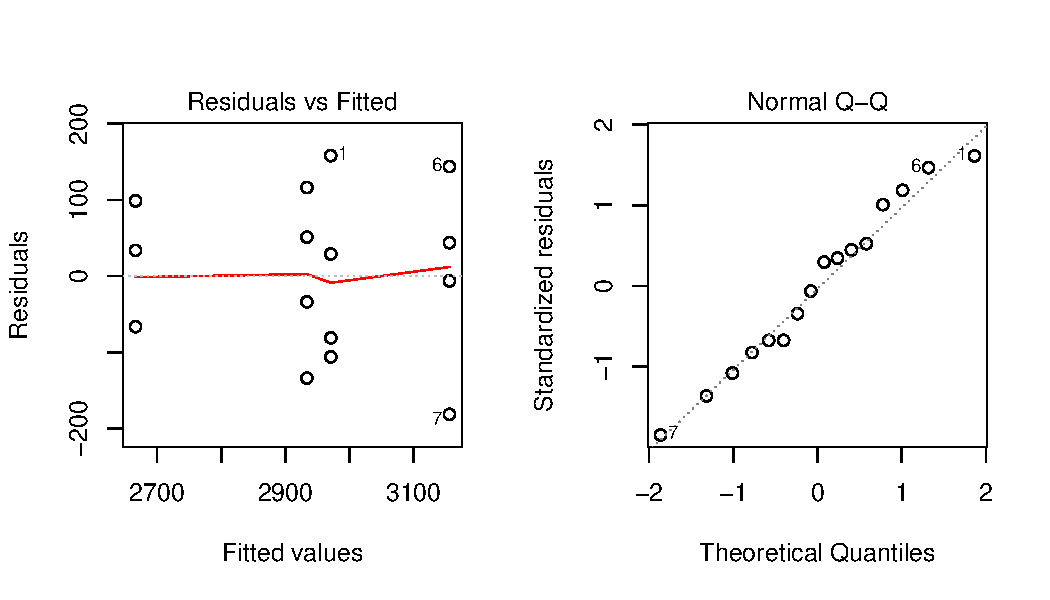
\includegraphics[width=\maxwidth]{figures/plot-t3-anova-1} 

}



\end{knitrout}

Before interpreting the results, we first examine the validity of the model assumptions about the errors. The Tukey-Anscombe plot shows that there are no major deviations from the zero-mean and homoscedasticity assumptions on the errors, and the Normal QQ-plot doesn't show any apparent deviation from the normality assumption on the errors. Therefore, we can conclude that the assumptions about the model are not refuted by the residual analysis, and we can proceed to interpret the results.

From the summary we can see that the F-statistics is 12.73, which is quite large for F-distribution with 3 and 12 degrees of freedom. This is also evident from the p-value being 0.0005, which is very small and we would therefore reject the null hypothesis that the group means are all the same. Therefore, we can conclude there is strong evidence that for at least one mixing technique, the mean compressive strength differs from others. However, we cannot conclude much more from the global F-test. To yield more information about where the differences come from, we perform the multiple pairwise-comparison, to determine if the differences in the means between specific group pairs are statistically significant. \\

As the ANOVA test is significant, we can compute Tukey Honest Significant Differences for performing multiple pairwise-comparison between the group means. We use Tukey HSD method which accounts for multiple testing correction as now we have more simultaneous tests and we have to account for that. For fitting, we use the function \verb+glht()+ [in \verb+multcomp+ package], where glht stands for general linear hypothesis tests.

\begin{knitrout}
\definecolor{shadecolor}{rgb}{0.969, 0.969, 0.969}\color{fgcolor}\begin{kframe}
\begin{alltt}
\hlkwd{library}\hlstd{(multcomp)}
\hlkwd{summary}\hlstd{(}\hlkwd{glht}\hlstd{(fit,} \hlkwc{linfct} \hlstd{=} \hlkwd{mcp}\hlstd{(}\hlkwc{mixing} \hlstd{=} \hlstr{"Tukey"}\hlstd{)))}
\end{alltt}
\begin{verbatim}
## 
## 	 Simultaneous Tests for General Linear Hypotheses
## 
## Multiple Comparisons of Means: Tukey Contrasts
## 
## 
## Fit: aov(formula = strength ~ mixing, data = X)
## 
## Linear Hypotheses:
##            Estimate Std. Error t value Pr(>|t|)    
## 2 - 1 == 0   185.25      80.08   2.313   0.1495    
## 3 - 1 == 0   -37.25      80.08  -0.465   0.9653    
## 4 - 1 == 0  -304.75      80.08  -3.806   0.0116 *  
## 3 - 2 == 0  -222.50      80.08  -2.778   0.0692 .  
## 4 - 2 == 0  -490.00      80.08  -6.119   <0.001 ***
## 4 - 3 == 0  -267.50      80.08  -3.340   0.0262 *  
## ---
## Signif. codes:  0 '***' 0.001 '**' 0.01 '*' 0.05 '.' 0.1 ' ' 1
## (Adjusted p values reported -- single-step method)
\end{verbatim}
\end{kframe}
\end{knitrout}

In the output we can see the individual comparisons between all groups with the p-value being adjusted for multiple testing such that in controls for the family-wise error rate. We can see that the largest difference is between mixing techniques 4 and 2, where the estimate for the difference between those two is $-490$ with p-value being significant at all levels. The differences between mixing techniques 4 - 1 and 4 - 3 are also significant at level 0.05. With the estimated difference between both of them are negative, we can conclude that the mixing technique 4 has significantly smallest compressive strength out of the mixing techniques considered.

Hence, the answer to the main question in this task is yes, there is evidence in the data that the mixing technique does affect the compressive strength of the concrete, and more specifically, based on further analysis, we would not recommend the use mixing technique 4 for concrete in practice.

\section*{Task 4}
Consider the data set munich.csv. The data set contains information on therent prices of apartments in Munich.  The variables in the data set are:

\begin{itemize}
\item rent:  net rent per month (in Euro) \\
\item area:  living area in square meters \\
\item yearc: year of construction \\
\item location:  quality of location according to an expert assessment (0 = average, 1 = good, 2 = top)
\end{itemize}

1) Here we read the data into R and interpret the location variable as factor. Furthermore we visualize the data by showing relation of each variable to the predicted variable rent.
\begin{knitrout}
\definecolor{shadecolor}{rgb}{0.969, 0.969, 0.969}\color{fgcolor}\begin{kframe}
\begin{alltt}
\hlstd{munich} \hlkwb{<-} \hlkwd{read.csv}\hlstd{(}\hlstr{"munich.csv"}\hlstd{)}
\hlstd{munich}\hlopt{$}\hlstd{location} \hlkwb{<-} \hlkwd{factor}\hlstd{(munich}\hlopt{$}\hlstd{location)}
\end{alltt}
\end{kframe}
\end{knitrout}


\begin{knitrout}
\definecolor{shadecolor}{rgb}{0.969, 0.969, 0.969}\color{fgcolor}

{\centering 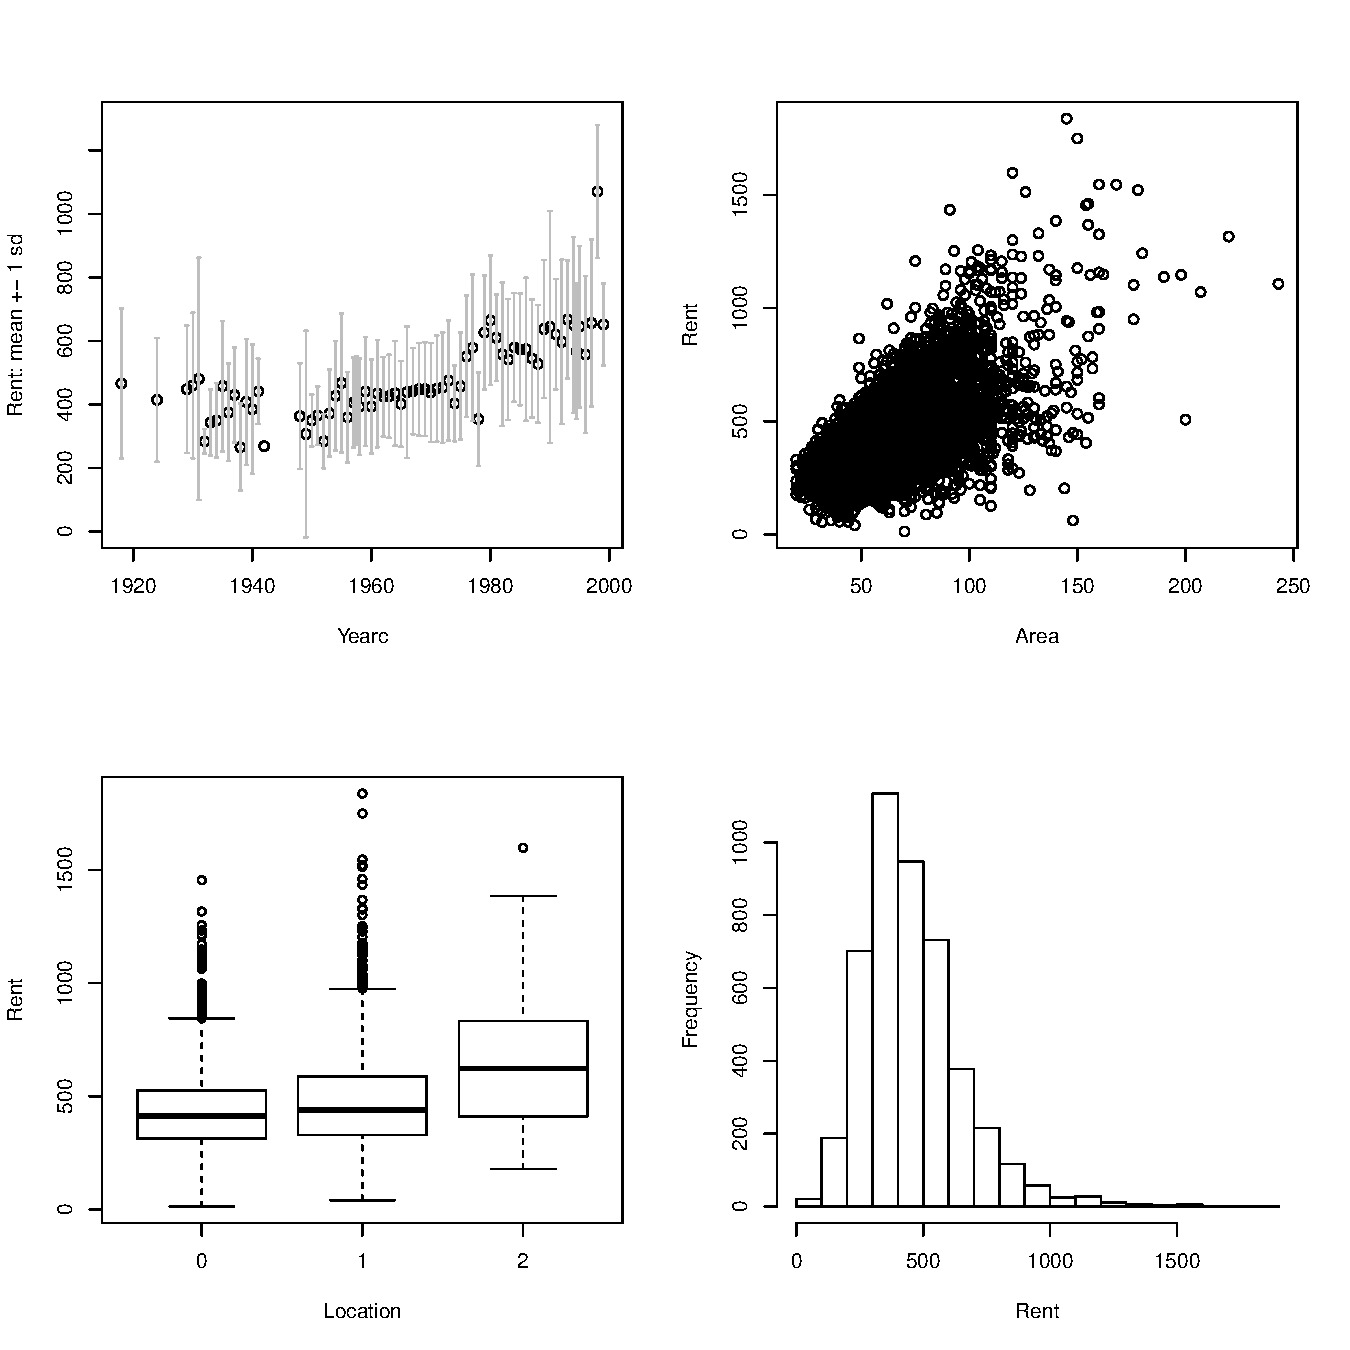
\includegraphics[width=\maxwidth]{figures/plot-t4-discuss-1} 

}



\end{knitrout}
2)
From the above plots, we can already come to the reasonable conclusion that there is a relationship between variable rent and variables area, location and yearc, that could be well explained by the linear model. In other words, there seems to be a linear relationship between rent and variables area, location and yearc, which means that the linear model could be adequate for the analysis. To see whether the assumptions of the linear model hold, we analyse the resituals. The quality of the fit could be infered from the $R^2$ value. \\

3) Here, we estimate the model,
\[ Y = \beta_0 + \beta_1 X_{\text{area}}+ \beta_2 X_{\text{loc:good}} + \beta_3 X_{\text{loc:top}} + \beta_4 X_{\text{yearc}} + \beta_5 X_{\text{loc:good}} X_{\text{area}} + \beta_6 X_{\text{loc:top}}  X_{\text{area}} \]
\begin{knitrout}
\definecolor{shadecolor}{rgb}{0.969, 0.969, 0.969}\color{fgcolor}\begin{kframe}
\begin{alltt}
\hlstd{f1} \hlkwb{<-} \hlkwd{lm}\hlstd{(rent}\hlopt{~}\hlstd{area}\hlopt{*}\hlstd{location} \hlopt{+} \hlstd{yearc,} \hlkwc{data}\hlstd{=munich)}
\hlkwd{par}\hlstd{(}\hlkwc{mfrow}\hlstd{=}\hlkwd{c}\hlstd{(}\hlnum{2}\hlstd{,}\hlnum{2}\hlstd{)) ;} \hlkwd{plot}\hlstd{(f1)}
\end{alltt}
\end{kframe}

{\centering 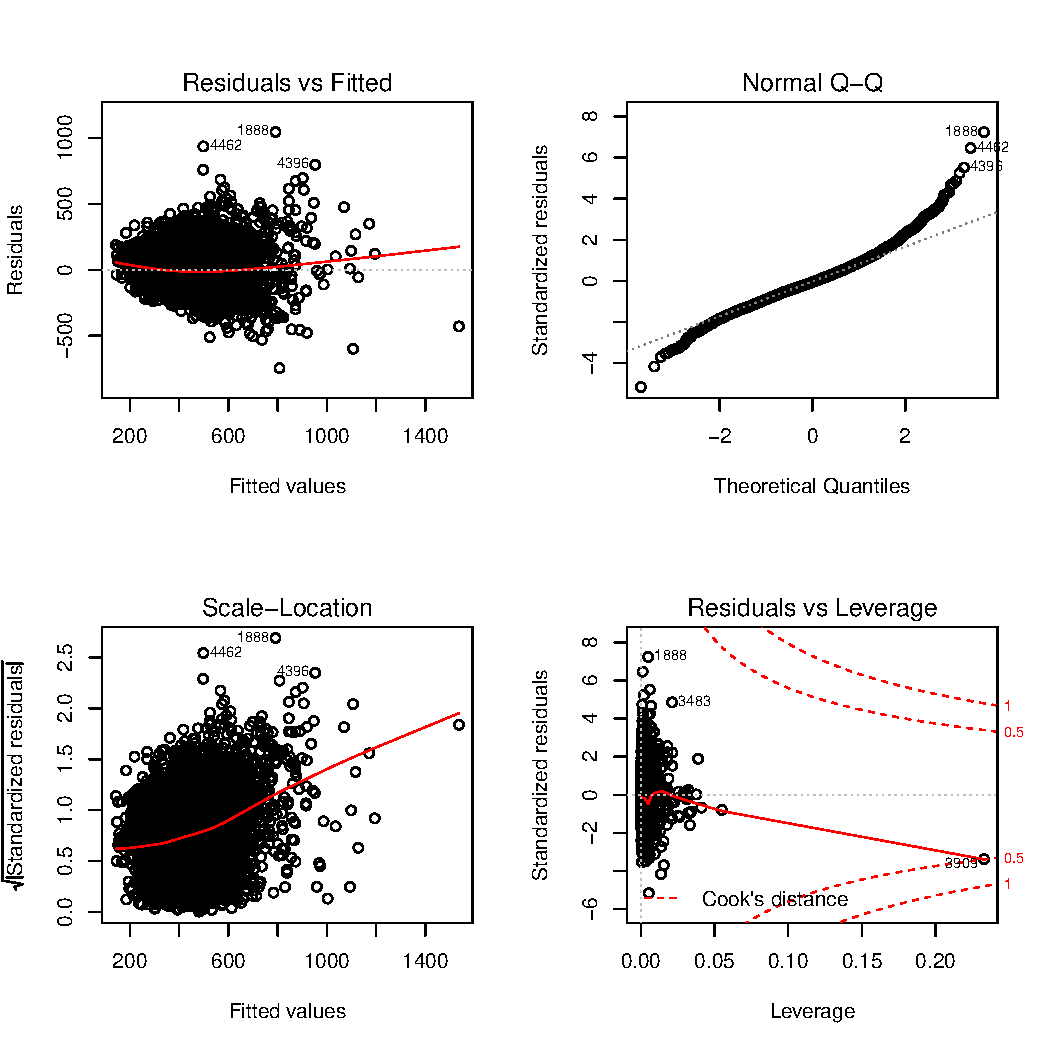
\includegraphics[width=\maxwidth]{figures/plot-t4-model-1} 

}



\end{knitrout}

4) From the 'Residuals vs Fitted' plot in the top left, we see that the assumption of zero-mean errors does not have major violations. There is some deviation as the trend line drifts away from zero for larger fitted values, but this can be explained by the lack of data in that area of the plot. \\

The 'Normal Q-Q' plot is concerning because the residuals show right-skewed distribution rather than normal. The deviation is not extremely severe, however, there is valid evidence against the normality assumption. \\

In the 'Scale-Location' graph, we see a clear violation of the homoscedasticity assumption as we have evidence for heteroscedastic residuals because the trend variance of residuals appears to get larger as the fitted values get larger (which we can also observe in the first plot). It could be argued again that this deviation of the trend line from the expected behaviour is partly due to having just a few datapoints in that area of the plot, but here the evidence of violation is substantial even in parts where we have sufficient data.\\

Finally, in the 'Residuals vs Leverage' plot we can see that the majority of the datapoints have low leverage and a relatively small Cook's distance. There is just one point, in row 3909, which has a high leverage as well as a high Cook's distance. This datapoint is borderline influential as its Cook's distance is around 0.5, and it should be looked at in more detail as the analysis progresses beyond this initial phase.\\

The conclusion from the residual analysis is that there are issues with the assumptions of the linear model with respect to the homoscedasticity assumption and also with respect to the normality assumption. A very good idea in this case would be to look at the variables and perform a log-transformation on the right-skewed variables. Log-transformation can stabilize the variance and solve the heteroscedasticity issue, and also it can deal with the right-skewed distribution by bringing it closer to the normal distribution. So, the log-transformation could potentially solve both problems, and we will address this later. \\

5) Below we display and interpret the model results.
\begin{knitrout}
\definecolor{shadecolor}{rgb}{0.969, 0.969, 0.969}\color{fgcolor}\begin{kframe}
\begin{alltt}
\hlkwd{summary}\hlstd{(f1)}
\end{alltt}
\begin{verbatim}
## 
## Call:
## lm(formula = rent ~ area * location + yearc, data = munich)
## 
## Residuals:
##     Min      1Q  Median      3Q     Max 
## -746.56  -86.86   -8.91   78.91 1046.26 
## 
## Coefficients:
##                  Estimate Std. Error t value Pr(>|t|)    
## (Intercept)    -5.356e+03  1.964e+02 -27.274  < 2e-16 ***
## area            4.732e+00  1.267e-01  37.344  < 2e-16 ***
## location1      -1.052e+00  1.302e+01  -0.081 0.935595    
## location2       1.219e+01  3.858e+01   0.316 0.752029    
## yearc           2.796e+00  9.971e-02  28.036  < 2e-16 ***
## area:location1  6.948e-01  1.802e-01   3.855 0.000117 ***
## area:location2  1.519e+00  4.449e-01   3.414 0.000646 ***
## ---
## Signif. codes:  0 '***' 0.001 '**' 0.01 '*' 0.05 '.' 0.1 ' ' 1
## 
## Residual standard error: 144.9 on 4564 degrees of freedom
## Multiple R-squared:  0.4575,	Adjusted R-squared:  0.4568 
## F-statistic: 641.5 on 6 and 4564 DF,  p-value: < 2.2e-16
\end{verbatim}
\end{kframe}
\end{knitrout}

The model results confirm our reasoning that there is a linear relationship between the variable rent and the three variables (area, location, and yearc). Both area and yearc have a very low p-value which means that there is strong evidence that they have a linear association with the outcome variable rent. Location has a high p-value which would at first glance suggest that it doesn't have a significant relationship with the rent value, however we can see that the interaction between location and area has a low p-value, so it is possible that the 'information' given by location is captured in this interaction. It is a good practice to leave the 'main effect' of the variable in the model when its interaction with another variable is included, so we keep the variable location because of its interaction with area.\\

6) First we fit a linear model including only the variable $area$ and display the results.
\begin{knitrout}
\definecolor{shadecolor}{rgb}{0.969, 0.969, 0.969}\color{fgcolor}\begin{kframe}
\begin{alltt}
\hlstd{f2} \hlkwb{<-} \hlkwd{lm}\hlstd{(rent}\hlopt{~}\hlstd{area,} \hlkwc{data}\hlstd{=munich)}
\hlkwd{summary}\hlstd{(f2)}
\end{alltt}
\begin{verbatim}
## 
## Call:
## lm(formula = rent ~ area, data = munich)
## 
## Residuals:
##     Min      1Q  Median      3Q     Max 
## -774.37  -99.85   -7.31   89.87 1016.36 
## 
## Coefficients:
##              Estimate Std. Error t value Pr(>|t|)    
## (Intercept) 135.63725    6.89211   19.68   <2e-16 ***
## area          4.73031    0.09541   49.58   <2e-16 ***
## ---
## Signif. codes:  0 '***' 0.001 '**' 0.01 '*' 0.05 '.' 0.1 ' ' 1
## 
## Residual standard error: 158.6 on 4569 degrees of freedom
## Multiple R-squared:  0.3498,	Adjusted R-squared:  0.3496 
## F-statistic:  2458 on 1 and 4569 DF,  p-value: < 2.2e-16
\end{verbatim}
\end{kframe}
\end{knitrout}

We can see that the adjusted $R^2$ coefficient for this model is only $0.35$, whereas for the model before it had value $0.46$. Note that we use adjusted $R^2$ so that we can compare models with different number of variables. Since the smaller model is nested within the bigger one, we can also compare the model using analysis of variance.

\begin{knitrout}
\definecolor{shadecolor}{rgb}{0.969, 0.969, 0.969}\color{fgcolor}\begin{kframe}
\begin{alltt}
\hlkwd{anova}\hlstd{(f2, f1)}
\end{alltt}
\begin{verbatim}
## Analysis of Variance Table
## 
## Model 1: rent ~ area
## Model 2: rent ~ area * location + yearc
##   Res.Df       RSS Df Sum of Sq      F    Pr(>F)    
## 1   4569 114891462                                  
## 2   4564  95857954  5  19033509 181.25 < 2.2e-16 ***
## ---
## Signif. codes:  0 '***' 0.001 '**' 0.01 '*' 0.05 '.' 0.1 ' ' 1
\end{verbatim}
\end{kframe}
\end{knitrout}

This analysis shows that the larger model with area, location, yearc, and the interaction between area and location is significantly better than the smaller model with just area. The Residual Sum of Squares is significantly lower, leading to a very low p-value that gives a significant result and a very strong evidence against the null hypothesis that the coefficients on location, yearc and area:location are all equal to zero simultaneously.

\pagebreak

7) Additional imporvement to the model with the log-transformation:

\begin{knitrout}
\definecolor{shadecolor}{rgb}{0.969, 0.969, 0.969}\color{fgcolor}\begin{kframe}
\begin{alltt}
\hlkwd{par}\hlstd{(}\hlkwc{mfrow} \hlstd{=} \hlkwd{c}\hlstd{(}\hlnum{1}\hlstd{,}\hlnum{3}\hlstd{))}
\hlkwd{hist}\hlstd{(munich}\hlopt{$}\hlstd{rent)}
\hlkwd{hist}\hlstd{(munich}\hlopt{$}\hlstd{area)}
\hlkwd{hist}\hlstd{(munich}\hlopt{$}\hlstd{yearc)}
\end{alltt}
\end{kframe}

{\centering 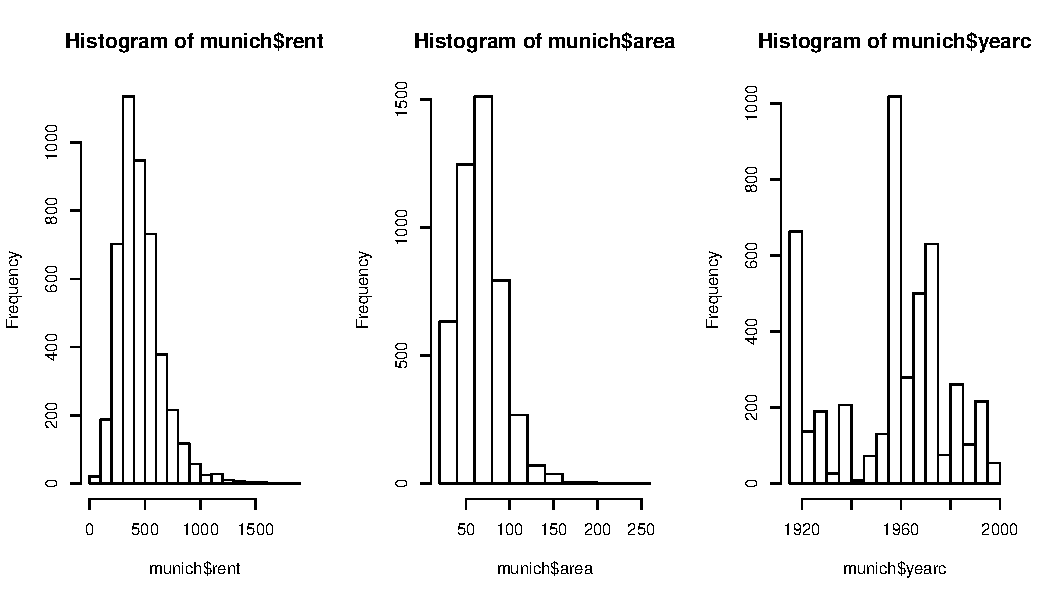
\includegraphics[width=\maxwidth]{figures/plot-t4-logtransform-1} 

}



\end{knitrout}

The histograms indicate that we could benefit from the log-transformation on rent and area.

\begin{knitrout}
\definecolor{shadecolor}{rgb}{0.969, 0.969, 0.969}\color{fgcolor}\begin{kframe}
\begin{alltt}
\hlstd{f3} \hlkwb{<-} \hlkwd{lm}\hlstd{(}\hlkwd{log}\hlstd{(rent)}\hlopt{~}\hlkwd{log}\hlstd{(area)}\hlopt{*}\hlstd{location} \hlopt{+} \hlstd{yearc,} \hlkwc{data}\hlstd{=munich)}
\hlkwd{par}\hlstd{(}\hlkwc{mfrow}\hlstd{=}\hlkwd{c}\hlstd{(}\hlnum{2}\hlstd{,}\hlnum{2}\hlstd{))}
\hlkwd{plot}\hlstd{(f3)}
\hlkwd{summary}\hlstd{(f3)}
\end{alltt}
\begin{verbatim}
## 
## Call:
## lm(formula = log(rent) ~ log(area) * location + yearc, data = munich)
## 
## Residuals:
##     Min      1Q  Median      3Q     Max 
## -3.6814 -0.1748  0.0336  0.2128  1.1602 
## 
## Coefficients:
##                       Estimate Std. Error t value Pr(>|t|)    
## (Intercept)         -8.9657903  0.4561628 -19.655  < 2e-16 ***
## log(area)            0.6690205  0.0181359  36.889  < 2e-16 ***
## location1           -0.1300419  0.1127515  -1.153  0.24883    
## location2           -0.7092476  0.3380585  -2.098  0.03596 *  
## yearc                0.0062252  0.0002264  27.493  < 2e-16 ***
## log(area):location1  0.0546899  0.0270535   2.022  0.04328 *  
## log(area):location2  0.2176273  0.0778930   2.794  0.00523 ** 
## ---
## Signif. codes:  0 '***' 0.001 '**' 0.01 '*' 0.05 '.' 0.1 ' ' 1
## 
## Residual standard error: 0.3301 on 4564 degrees of freedom
## Multiple R-squared:  0.4134,	Adjusted R-squared:  0.4127 
## F-statistic: 536.2 on 6 and 4564 DF,  p-value: < 2.2e-16
\end{verbatim}
\end{kframe}

{\centering 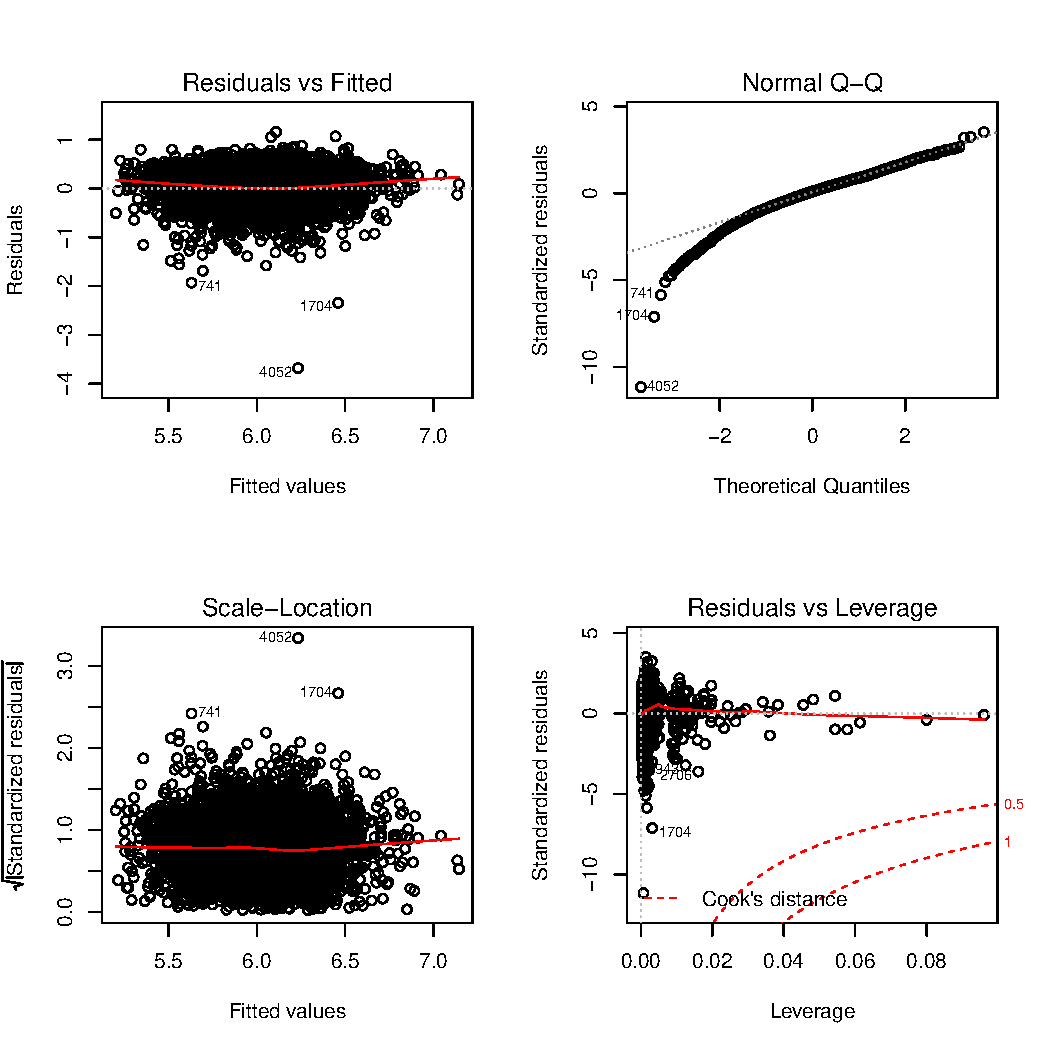
\includegraphics[width=\maxwidth]{figures/plot-t4-logfit-1} 

}



\end{knitrout}

The residual analysis seems much better and the heteroscedasticity issue is resolved. There is a minor problem again with the QQ-plot because now the residuals show left-skewed distribution. However, left-skew creates less problems than the right-skew, and it also seems less severe than before. The analysis shows that all of the variables are significant now, however, the R-squared has slightly dropped compared to the previous analysis. In conclusion, the log-transformation does not yield a better fit in terms of explaining the variance in rent, but it does substantially improve the violations of the linear model's assumptions, especially heteroscedasticity which is non-existent after the transformation.

\end{document}
